\documentclass{article}
\usepackage[utf8]{inputenc}
\usepackage{amsmath}
\usepackage{physics}
\usepackage{simplewick}
\usepackage{graphicx}
\usepackage{appendix}
\usepackage[backend=biber,style=nature]{biblatex}
\addbibresource{library.bib}
\usepackage[margin=1.6in]{geometry}
\usepackage{booktabs}

\usepackage[affil-it]{authblk} 
\usepackage{etoolbox}
\usepackage{lmodern}

\usepackage{xr}
\makeatletter
\newcommand*{\addFileDependency}[1]{% argument=file name and extension
  \typeout{(#1)}
  \@addtofilelist{#1}
  \IfFileExists{#1}{}{\typeout{No file #1.}}
}
\makeatother
 
\newcommand*{\myexternaldocument}[1]{%
    \externaldocument{#1}%
    \addFileDependency{#1.tex}%
    \addFileDependency{#1.aux}%
}
\myexternaldocument{sup}

\makeatletter
\patchcmd{\@maketitle}{\LARGE \@title}{\fontsize{16}{19.2}\selectfont\@title}{}{}
\makeatother

\renewcommand\Authfont{\fontsize{12}{14.4}\selectfont}
\renewcommand\Affilfont{\fontsize{9}{10.8}\itshape}

% \title{Simulation of TEM-induced electronic excitation in crystalline solids}
\title{\textbf{Electron beam-induced excitation rates in crystalline solids from first-principles}}
\author[1,2]{Anthony Yoshimura}
\author[2]{Michael Lamparski}
\author[2]{Joel Giedt}
\author[3]{David Lingerfelt}
\author[3]{Jacek Jakowski}
\author[3]{Ganesh Panchapakesan}
\author[4]{Tao Yu}
\author[4]{\\Bobby Sumpter}
\author[2,5*]{Vincent Meunier}
\affil[1]{Design Physics Division, Lawrence Livermore National Laboratory, Livermore, CA 94550, USA}
\affil[2]{Department of Physics, Applied Physics, and Astronomy, Rensselaer Polytechnic Institute, Troy, New York 12180, USA}
\affil[3]{Computational Sciences and Engineering Division, Oak Ridge National Laboratory, Oak Ridge, TN 37831, USA}
\affil[4]{Department of Chemistry, University of North Dakota, Grand Forks, ND 58202, USA}
\affil[5]{Department of Materials Science and Engineering, Rensselaer Polytechnic Institute, Troy, NY 12180, USA}
\affil[*]{Correspondence to be addressed to meuniv@rpi.edu}

\begin{document}

\maketitle

\begin{abstract}
% context
The ability to control the structure of any material at the atomic-scale can provide powerful solutions to many of today’s most pressing technological and environmental challenges. To this end, electron irradiation by transmission electron microscopy can be used to engineer the morphology of 2-dimensional (2D) materials with a high degree of spatial control.
It follows that many computational models have been developed to predict the rates of atomic displacements in irradiated materials.
% Need
However, while current models give reasonable predictions for conductors, they often drastically underestimate the displacement rates in insulators.  This is because the majority of these methods focus solely on interactions between the beam electrons and target nuclei, neglecting the possibility of beam-induced electronic excitations.
In insulators, these excitations can reduce the binding energies of the irradiated atoms, increasing their displacement rates.
% Task / Document
To address this phenomenon, this paper combines quantum electrodynamics with density functional theory to calculate the probability of beam-induced of excitation in 2D insulating crystals.
% Findings
We find that the probability of excitation induced by the transmission of a single 60 keV beam electron is about 16\% in hexagonal boron nitride and 67\% in molybdenum disulfide.
% is about 19\% 60 keV, and scales inversely to the beam energy.
These probabilities increase and approach unity as the beam energy approaches zero.
% This model can also generate electron energy loss spectra.
% Conclusions
Incorporating these probabilities into computational models 
% greatly increases the predicted rate of atomic displacement, 
reveals that appreciable sputtering can occur at beam energies much lower than we would otherwise expect,
reducing the disparity between theory and experiment.
% perspective
This new predictive power would be a boon for materials engineers, allowing for the controlled manipulation of any 2D material for targeted functionality.
\end{abstract}
    
%------------------------------------------------------------------------------
\section{Introduction}
\label{sec:intro}
%------------------------------------------------------------------------------

% Context: orient the readers who are less familiar with the topic to establish importance of the work
A game a billiards involves two types of collisions: ball-to-ball and ball-to-table. In a ball-to-ball collision, the energy transfer from the moving ball to the stationary ball can be large because their masses are equal.  It follows that a set of initially stationary balls are expected to rearrange after ball-to-ball collisions.  One could call such collisions \textit{inelastic}, since they cause the initially moving ball to lose a significant amount of its energy.
On the other hand, very little energy is transferred in a ball-to-table collision, in which a moving ball strikes the rail of the table.  This is because the mass of the table is much greater than that of the ball.  As a result, the ball is expected to bounce off the rail without losing any velocity.  In this way, one could call such a collision \textit{elastic}, since the moving ball retains its energy.

In the case of a material under electron beam irradiation, electron-electron collisions liken to ball-to-ball, while electron-nuclear collisions liken to ball-to-table.  As such
% we can be very confident that the electrons will rearrange immediately after the collision.
we expect the material electrons to rearrange quite readily from an inelastic collision with the beam electron.  This rearrangement comes in the form of electronic excitation.
% whether or not these excitations are long-lived enough to be measured is a different story
These beam-induced excitations are prevalent and consequential.  They can affect the materials structural response to an irradiating electron beam.
% It is therefore widely recognized that electron-electron interactions should not be ignored when
\begin{enumerate}
\item
There are a variety of structural responses that can take place under electron irradiation.  In this work, we focus solely on \textit{sputtering}, in which an atom is ejected from the material, leaving behind a vacancy.  Sputtering results from electron-nuclear collisions.  If the energy transferred to the nucleus is greater than its displacement threshold $E_d$, it will sputter.
\item 
critical energy is the minimum beam energy required to sputter an atom, assuming the atom is initially at rest.
\item
2D materials provide an excellent platform to track displacement rates under electron irradiation.  2D materials have many distinct and interesting properties.
They are also a perfect platform to test displacement cross sections.
\end{enumerate}
Defects in materials are interesting.
While defects will almost certainly destroy the properties of the pristine material, they can vastly extend the the space of possible applications.
Electron irradiation by transmission electron microscopy (TEM) is an effective method for engineering the properties and morphology of an irradiated material with sub-angstrom precision via selective atomic displacement \cite{Zhao2017, Schleberger2018,Oxley2014,Kretschmer2018,Komsa2013}.
% Need:
Many computational models have been proposed to predict electron beam-induced displacement rates in 2D materials  \cite{Meyer2012, Susi2016, Yoshimura2018, Susi2019}. However, the vast majority of current methods focus solely on interactions between the beam electrons and target nuclei, neglecting any coupling with the material’s electrons.  Thus, while present-day models give reasonable predictions for conductors, where electronic relaxation is rapid, they often vastly underestimate the atomic displacement rates in insulators.
For example, boron has been shown to sputter from hexagonal boron nitride (hBN) under irradiation that is about half of the calculated critical energy \cite{Susi2019, Cretu2015}.  Furthermore, Se sputters from WSe$_2$ under irradiation of 60 keV, almost 150 keV below its predicted critical energy \cite{Lin2015}.  Perhaps even more surprising is that chalcogen sputtering rates in MoS$_2$ and MoSe$_2$ were observed to be about equal under 80 keV irradiation \cite{Lehnert2017}, despite Se being more than two times heavier than S.
Discrepancies in semiconductors like these severely inhibit the use of TEM for materials engineering, as electronic energy gaps are the foundation of electronic and photoelectric device technology. 

% It is a stretch to claim we have a high-precision method if the displacement rate is orders of magnitude larger than the callibration.

% Task: what you have done to address the need
These results suggest that the displacement thresholds in insulating crystals are much smaller than what is predicted by ground state DFT.  Lehnert et al. \cite{Lehnert2017} have proposed that the consideration of inelastic scattering, i.e., beam-induced electron excitation, can lead to a reduction in $E_d$.   This would increase the sputtering rates and enable sputtering under beam energies well-below the ground state critical energy.
In light of this, this work combines quantum electrodynamics (QED) and density functional theory (DFT) to derive the probability of beam-induced excitation in 2D insulating crystals.
% The basic idea is this:
DFT can provide effective single particle states that can be decomposed into a plane wave basis \cite{Hohenberg1964,Kohn1965,Kresse1996a}, while QED is well-equipped to describe how each plane wave evolves in time through interactions with an electromagnetic field \cite{Peskin1995,Lancaster2014}. Thus, a plane wave decomposition of the Kohn-Sham orbitals can allow for a component-by-component treatment of the interactions between the beam and material electrons.  This generalized QED-DFT approach will enable, for the first time, a first-principles description of any beam-matter interaction process, with the only approximation being the order in the fine-structure constant to which the time-evolution operator is expanded.
% Object: preview the remainder of the paper to mentally prepare readers for its structure
This paper is divided into two sections: First, we derive the probability of an excitation for a 2D insulating crystal as a function of beam energy. Second, we show how this excitation probability can be used to predict sputtering rates in insulators.

% In this work, we lay out a method with which we can predict a material's structural response to electron beam irradiation.
% This new model would be a boon for materials science, allowing for the controlled atomic-scale manipulation of any material for targeted functionality.
% Experiment has shown that the Rutherford and MF cross sections drastically underestimate the sputtering rates in semiconducting 2D materials.
% demonstrate how the consideration of electron-electron scattering can lead to the prediction of significantly higher sputtering rates in gapped materials, closing the disparity between theory and experiment.

%------------------------------------------------------------------------------
\section{Probability of beam-induced excitation}
\label{sec:probability}
%------------------------------------------------------------------------------
The sputtering of an excited atom hinges on three successive processes.
(1)
A beam electron excites $n$ ground state electrons to unoccupied states.
% reducing the displacement threshold of the affected atom to $E_d^n$;
(2)
The energy $E_t$ transferred to that atom's nucleus by the beam electron is greater than the displacement threshold $E_d(n)$, which depends on the number of excitations
(3)
The excited electron remains excited long enough for the target atom to leave the vicinity of its original site.
% for a given number of;
% Thus, the probability of sputtering is
Thus, the total sputtering cross section
% is facilitated by electronic-excitation
can be written as
% the product of three probabilities

\begin{equation}
\label{eq:threeProbs}
    % P(\text{sputtering})
    \sigma(\text{sputtering})
    =
    % P(\text{excitation})
    \sum_{n=1}
    P_\text{ex}(E_b)
    \times P(\text{still excited})
    % \times P(E_t > E_d)
    \times \sigma\left(E_t > E_d(n)\right)
    .
\end{equation}
%
The method for calculating $P(E_t > E_d)$ for a given temperature well-established in the literature \cite{Meyer2012,Susi2016,Yoshimura2018}.  Meanwhile, first-principles methods for calculation of $P(\text{still excited})$ have already been established, and often, experimental data can be used to determine the excitation lifetimes in a material.  Therefore, this section focuses on how to obtain $P(\text{excitation})$ by combining QED and DFT.

% In this section, we derive an expression for $P(\text{excitation})$.  
% We start by describing the basic mechanism for beam induced electronic excitation.
In a ground state crystal, an occupied electron energy eigenstate has zero overlap with any unoccupied state.  As energy eigenstates are stationary, this means that an electron in an occupied state will never be measured in an excited state if left unperturbed.  However, the collision of a beam electron can give an occupied state a momentum boost that breaks its orthogonality with the unoccupied states.  Thus, the boosted ground state state has a nonzero probability of being measured in an excited state.  This is the basic mechanism of beam-induced excitation.

With this in mind, the method for deriving the excitation probability proceeds as follows:
First,
% determine the amplitude for a beam electron to boost an electron in a momentum eigenstate into another momentum eigenstate. 
determine the amplitude for a free electron to scatter from one momentum eigenstate into another after collision with another free electron.
Second,
% use the free electron scattering amplitude to derive the amplitude for the scattering of arbitrary wavepackets.  To
obtain the amplitude for scattering from one wavepacket into another by summing over the amplitudes for each momentum component of one wave packet to scatter into each momentum component of the other.
Third,
decompose a pair of occupied and unoccupied crystal states into a momentum basis and plug them in as the incoming and outgoing wave packets respectively.  Square the amplitude to obtain the corresponding excitation probability
Finally,
find the probability of not exciting any transitions and subtract that probability from unity.  The result is the probability of exciting at least one crystal electron.

%------------------------------------------------------------------------------
\subsection{Scattering of free electrons}
\label{sec:ee}
%------------------------------------------------------------------------------

\begin{figure}
    \centering
    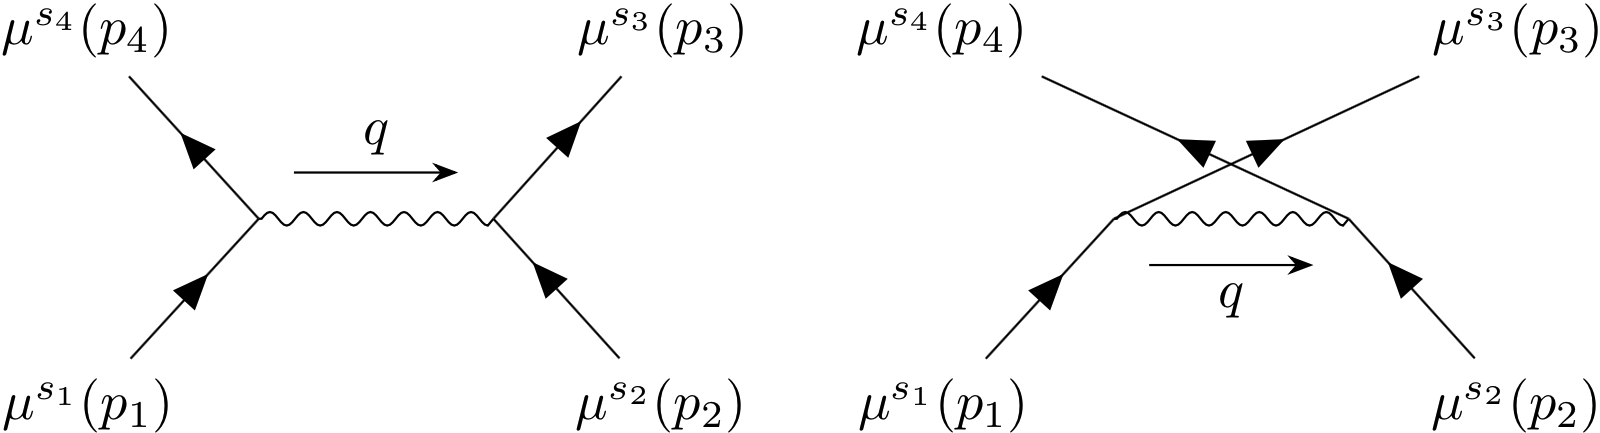
\includegraphics[width=.8\textwidth]{images/tu.png}
    \caption{
    The lowest order electron-electron scattering perturbation includes two Feynmann diagrams: the $t$-channel (left) and the $u$-channel (right).
    }
    \label{fig:tu}
\end{figure}

We first derive the scattering amplitude for momentum transfer between two free electrons.
Going forward, we label the 4-momenta of the incoming electrons as $p_1$ and $p_2$, while the outgoing electrons have momenta $p_3$ and $p_4$.
The 4-momentum of the $n$th electron can be written as
$p_n = (\epsilon_n, p_n^x, p_n^y, p_n^z) = (\epsilon_n, \mathbf{p}_n)$
%\begin{equation}
%    p= (p^0, p^x, p^y, p^z) = (p^0, \mathbf{p}),
%\end{equation}
%
% where $\epsilon_\mathbf{p}^2 = |\mathbf{p}|^2 + m^2$.
where $\epsilon_n$ is the particle's energy and $\mathbf{p}_n$ is its 3-momentum.
% Moving forward, italicized letters will often denote 4-vectors, e.g. $p = (p^0, p^x, p^y, p^z)$, while boldface letters will denote 3-vectors, e.g. $\mathbf{p} = (p^x, p^y, p^z)$.  Meanwhile,
Dot products between 4-vectors are taken over Minkowski space, i.e. $p_n\cdot p_m = g_{\mu\nu}p_n^\mu p_m^\nu = \epsilon_n\epsilon_m - \mathbf{p}_n\cdot\mathbf{p}_m$, where $\mathbf{p}_n\cdot\mathbf{p}_m = p_n^xp_m^x + p_n^yp_m^y + p_n^zp_n^z$.   

To lowest order, the amplitude for free electron scattering can be represented by two tree-level diagrams, which we call the $t$- and $u$-channels (figure \ref{fig:tu}).
% where there are two terms arising from two distinct sets of contractions.
% Note that the factor of 1/2 in equation (\ref{eq:SExpansion}) vanishes due to the fact that contracting $p_1$ with either $\hat{\psi}(x)$ or $\hat{\psi}(y)$ produces the same result.
% The two terms can be represented as two Feynman diagrams shown in figure \ref{fig:tu} , which we call the $t$- and $u$-channels.
% We can now use Wick's theorem to write the last expression in equation (\ref{eq:contraction}) in terms of Dirac spinors, as laid out in section \ref{app:wicks}. Doing this and integrating over $x$ and $y$ yields
Using Feynman's rules, we can write these diagrams in terms of Dirac spinors, yielding the invariant matrix element

\begin{equation}
\label{eq:M}
\begin{aligned}
    \mathcal{M}(p_4p_3\leftarrow p_2p_1)
    &=
    % \frac{1}{2}
    \frac{e^2}{2}
    \sum_{s_1}\sum_{s_2}\sum_{s_3}\sum_{s_4}
    \\&
    \bigg[
    \bar{u}^{s_4}\left(p_4\right)\gamma^{\mu}u^{s_1}\left(p_1\right)
    % D_{\mu\nu}(p_3 - p_2)
    % \frac{g_{\mu\nu}}{(p_3 - p_2)^2}
    \left(\frac{1}{p_3 - p_2}\right)^2
    % \bar{u}^{s_3}\left(p_3\right)\gamma^{\nu}u^{s_2}\left(p_2\right)
    \bar{u}^{s_3}\left(p_3\right)\gamma_{\mu}u^{s_2}\left(p_2\right)
    % \\&\qquad\qquad\qquad\qquad+
    \\&+
    \bar{u}^{s_3}\left(p_3\right)\gamma^{\mu}u^{s_1}\left(p_1\right)
    % D_{\mu\nu}(p_4 - p_2)
    % \frac{g_{\mu\nu}}{(p_4 - p_2)^2}
    \left(\frac{1}{p_4 - p_2}\right)^2
    \bar{u}^{s_4}\left(p_4\right)\gamma_{\mu}u^{s_2}\left(p_2\right)
    \bigg]
\end{aligned}
\end{equation}
%
where $s_n = 1\text{ or }2$ denotes the spin of the $n$th electron.  The factor of 1/2 before the summation arises from the assumption that the incoming states are unpolarized.  The last line of equation (\ref{eq:M}) defines the invariant matrix element $\mathcal{M}$.
% (squaring and spin averaging this $\mathcal{M}$ gives the M{\o}ller cross section).
% In the last line, we define the invariant matrix element $\mathcal{M}$ as the sum of these two terms.
The evaluation of $\mathcal{M}$ in terms of the components of the electron 4-momenta is straightforward, though cumbersome, and is described in section \ref{app:M}.

The momentum transfer is $p_3 - p_2$ for the $t$-channel and $p_4 - p_2$ for the $u$-channel.  Because the DFT cutoff energy is much smaller than the beam energy, we only consider momentum transfers that are much smaller than $p_1$.  This means that one channel is always much bigger than the other.  Taking advantage of the indistinguishibility of the electrons, we calculate only the $t$-channel and multiply by 2 to obtain $\mathcal{M}$.
% Lastly, the tensor $D_{\mu\nu}(q)$ is the momentum-dependent photon-propagator, 

We can use $\mathcal{M}$ to quickly obtain the scattering amplitude between two free electrons

\begin{equation}
\label{eq:T}
    \bra{p_4 p_3}\hat{T}\ket{p_2p_1}
    =
    (2\pi)^4\delta(p_1 + p_2 - p_3 - p_4)
    \mathcal{M}(p_4p_3\leftarrow p_2p_1),
\end{equation}
%
where $\hat{T}$ is the scattering operator.
% The last line of equation (\ref{eq:spinors}) defines the invariant matrix element $\mathcal{M}$ (squaring and spin averaging this $\mathcal{M}$ gives the M{\o}ller cross section).
% In the last line, we define the invariant matrix element $\mathcal{M}$ as the sum of these two terms.
% Lastly, the tensor $D_{\mu\nu}(q)$ is the momentum-dependent photon-propagator, 

% \begin{equation}
% \label{eq:Dmunu}
    % D_{\mu\nu}(q) = \frac{-ig_{\mu\nu}}{q^2 + i\eta}    
% \end{equation}
%
% where $\eta \ll 1$ is a positive real number.  

%------------------------------------------------------------------------------
\subsection{Scattering of wavepackets}
\label{sec:wavepackets}
%------------------------------------------------------------------------------

%We drop the infinitesimal in section \ref{sec:ee} since $q^2$ is always nonzero.
% We see that the $t$-channel given in second line of equation (\ref{eq:spinors}) is equivalent to the $u$-channel given in the third line except for the swapping of indices 3 and 4.
% For the case of scattering from one crystal state to another, the amplitude that we are after is
% The amplitude for a beam electron to induce an electronic crystal excitation is given by

We can now determine the amplitude for the scattering of two arbitrary electron states
$\phi_1$ and $\phi_2$ into $\phi_3$ and $\phi_4$.

\begin{equation}
\label{eq:amp}
\begin{aligned}
    % &\bra{\Psi_f} \hat{T} \ket{\Psi_i}
    &\bra{\phi_4\phi_3} \hat{T} \ket{\phi_2\phi_1}
    % &\bra{p'_b, n'\mathbf{k'}} \hat{T} \ket{n\mathbf{k},p_b}
    =
    \int \frac{d^3p_4d^3p_3d^3p_2d^3p_1}
    {(2\pi)^{12} 16\epsilon_4\epsilon_3\epsilon_2\epsilon_1}
    % \bra{\Psi_f}\ket{p_4p_3}
    \bra{\phi_4\phi_3}\ket{p_4p_3}
    \bra{p_4p_3}\hat{T}\ket{p_2p_1}
    % \bra{p_2p_1}\ket{\Psi_i},
    % \bra{p_2p_1} \ket{n\mathbf{k},p_b}
    \bra{p_2p_1} \ket{\phi_2\phi_1}
\end{aligned}
\end{equation}
%
% where $\ket{\Psi_i}$ is an initial beam and valence electron state and $\ket{\Psi_f}$ is a final excited and scattered state.
On the right side, we have inserted two resolutions of the identity given in equation (\ref{eq:identity}) in the SI. By inserting equation (\ref{eq:T}), the amplitude can be written in terms of the invariant matrix element $\mathcal{M}$, becoming

\begin{equation}
\label{eq:ampPlugInM}
\begin{aligned}
    &\int\frac{d^3p_4d^3p_3d^3p_2d^3p_1}
    {(2\pi)^{12} 16\epsilon_4\epsilon_3\epsilon_2\epsilon_1}
    \bra{\phi_4}\ket{p_4}
    \bra{\phi_3}\ket{p_3}
    \bra{p_2}\ket{\phi_2}
    \bra{p_1}\ket{\phi_1}
    \\&\qquad\times
    \mathcal{M}(p_4p_3\leftarrow p_2p_1)
    (2\pi)^4\delta(p_1 + p_2 - p_3 - p_4).
\end{aligned}
\end{equation}
%
% where we have assumed that each of the incoming and outgoing electrons belongs to a state labelled $\phi_i$.
% The energy difference in the denominator of $\mathcal{M}$ is $q^0 = p_3^0 - p_2^0$ is the difference between eigenvalues $q^0 = \epsilon_{n'\mathbf{k'}} - \epsilon{n\mathbf{k}}$.
We can use the delta function to integrate over $\mathbf{p}_4$ and $p_3^z$, yielding

\begin{equation}
\label{eq:ampUseDelta}
\begin{aligned}
    \int\frac{d^2p_3^\perp d^3p_2d^3p_1}
    {(2\pi)^{8} 16\epsilon_2\epsilon_1}
    \frac{\mathcal{M}(p_4p_3\leftarrow p_2p_1)}
    % \frac{\mathcal{M}(p_4p_3\leftarrow p_2p_1)}
    {\left|p_3^z\epsilon_4 - p_4^z\epsilon_3\right|}
    \bra{\phi_4}\ket{p_4}
    \bra{\phi_3}\ket{p_3}
    \bra{p_2}\ket{\phi_2}
    \bra{p_1}\ket{\phi_1},
\end{aligned}
\end{equation}
%
where it is understood that $p_4$ and $p_3$ satisfy $p_1 + p_2 = p_3 + p_4$.
The normalization of 3-momentum states defined equation (\ref{eq:normalization}) allows us to rewrite the expression as

\begin{equation}
\label{eq:amp3Mom}
\begin{aligned}
    \int\frac{d^2p_3^\perp d^3p_2d^3p_1}{(2\pi)^{8}}
    \sqrt{\frac{\epsilon_4\epsilon_3}{\epsilon_2\epsilon_1}}
    % \frac{\mathcal{M}}
    \frac{\mathcal{M}(p_4p_3\leftarrow p_2p_1)}
    {4\left|p_3^z\epsilon_4 - p_4^z\epsilon_3\right|}
    \bra{\phi_4}\ket{\mathbf{p}_4}
    \bra{\phi_3}\ket{\mathbf{p}_3}
    \bra{\mathbf{p}_2}\ket{\phi_2}
    \bra{\mathbf{p}_1}\ket{\phi_1}.
\end{aligned}
\end{equation}
%
We can then discretize the momenta by replacing $d^3p_i/(2\pi)^3 \rightarrow V^{-1}$ and $d^2p_i^\perp/(2\pi)^2 \rightarrow A^{-1}$, where $V$ and $A$ are the volume and cross sectional area of the simulated crystal, i.e., the volume and cross sectional area of the unit cell times the number of k-points in the cell.  With this, the amplitude becomes

\begin{equation}
\label{eq:ampDisc}
\begin{aligned}
    \frac{1}{AV^2}
    \sum_{\mathbf{p}_3^\perp} \sum_{\mathbf{p}_2} \sum_{\mathbf{p}_1}
    \sqrt{\frac{\epsilon_4\epsilon_3}{\epsilon_2\epsilon_1}}
    % \frac{\mathcal{M}}
    \frac{\mathcal{M}(p_4p_3\leftarrow p_2p_1)}
    {4\left|p_3^z\epsilon_4 - p_4^z\epsilon_3\right|}
    \bra{\phi_4}\ket{\mathbf{p}_4}
    \bra{\phi_3}\ket{\mathbf{p}_3}
    \bra{\mathbf{p}_2}\ket{\phi_2}
    \bra{\mathbf{p}_1}\ket{\phi_1}.
\end{aligned}
\end{equation}
%
We are now ready to replace $\ket{\phi_1}$, $\ket{\phi_2}$, $\ket{\phi_3}$, and $\ket{\phi_4}$ with states relevant to electron beam-induced excitation.

%------------------------------------------------------------------------------
\subsection{probability of crystal excitations}
\label{sec:crystal}
%------------------------------------------------------------------------------

We now consider the specific case of beam-induced excitations
to determine the form of the four electron states in equation (\ref{eq:ampDisc}).
% $\ket{\phi_i}$
We assign $\ket{\phi_1}$ and $\ket{\phi_4}$ to the initial and final beam states $\ket{p_b}$ and $\ket{p'_b}$ respectively.  States $\ket{\phi_2}$ and $\ket{\phi_3}$ are then the ground and excited crystal states $\ket{n\mathbf{k}}$ and $\ket{n\mathbf{k'}}$ respectively.  The excitation amplitude becomes

\begin{equation}
\label{eq:crystalStates}
\begin{aligned}
    \bra{p'_b, n'\mathbf{k'}} \hat{T} \ket{n\mathbf{k},p_b}
    &=
    \frac{1}{AV^2}
    \sum_{\mathbf{p}_3^\perp} \sum_{\mathbf{p}_2} \sum_{\mathbf{p}_1}
    \sqrt{\frac{\epsilon_4\epsilon_3}{\epsilon_2\epsilon_1}}
    % \frac{\mathcal{M}}
    \frac{\mathcal{M}(p_4p_3\leftarrow p_2p_1)}
    {4\left|p_3^z\epsilon_4 - p_4^z\epsilon_3\right|}
    \\&\times
    \bra{\mathbf{p'}_b}\ket{\mathbf{p}_4}
    \bra{n'\mathbf{k'}}\ket{\mathbf{p}_3}
    \bra{\mathbf{p}_2}\ket{n\mathbf{k}}
    \bra{\mathbf{p}_1}\ket{\mathbf{p'}_b}.
\end{aligned}
\end{equation}
%
The zeroth components of the initial and final beam momenta obey the free particle dispersion relations, so that
$\epsilon_1 = \sqrt{|\mathbf{p}_1|^2 + m^2}$.
and
$\epsilon_4 = \sqrt{|\mathbf{p}_4|^2 + m^2}$.
Meanwhile, the momentum of the crystal states can be treated nonrelativistically.
Thus, the zeroth components of the crystal state momenta are the energy eigenvalues of their crystal states plus the electron rest mass, i.e., $\epsilon_2=\epsilon_{n\mathbf{k}} + m$ and $\epsilon_3=\epsilon_{n'\mathbf{k'}} + m$.

% We now consider the make-up of the four electron states  $\ket{\phi_i}$ for the case of a beam electron scatter off of a crystal electron.
We can now evaluate the overlaps in equation (\ref{eq:crystalStates}).
The initial beam state is highly localized on $\mathbf{p}_b$, meaning that
% probability density and corresponding amplitude of $\ket{\phi_1}$ can be approximated as

\begin{equation}
\label{eq:phi_1}
    % P(p_1)
    % =
    |\bra{\mathbf{p}_1}\ket{\mathbf{p}_b}|^2 = V\delta_{\mathbf{p}_1,\mathbf{p}_b}
    \quad\Rightarrow\quad
    \bra{\mathbf{p}_1}\ket{\mathbf{p}_b} = V^{1/2}\delta_{\mathbf{p}_1,\mathbf{p}_b}.
\end{equation}
%
Meanwhile, the ground and excited crystal states can be written as

\begin{equation}
\begin{aligned}
&\ket{n\mathbf{k}}
=
V^{-1/2}\sum_{\mathbf{G}} C_{\mathbf{G+k}}^n \ket{\mathbf{G+k}}
\\&
\ket{n'\mathbf{k'}}
=
V^{-1/2}\sum_{\mathbf{G'}} C_{\mathbf{G'+k'}}^{n'} \ket{\mathbf{G'+k'}},
\end{aligned}
\end{equation}
%
% where $n$ and $\mathbf{k}$ label the band and crystal momentum, and unprimed and primed variables label ground and excited states, respectively.  This means that
meaning that
\begin{equation}
\label{eq:phi_2}
\begin{aligned}
    &\bra{\mathbf{p}_2}\ket{\phi_2}
    =
    \bra{\mathbf{G + k}}\ket{n\mathbf{k}}
    =
    V^{1/2}C^n_\mathbf{G+k}
    \\&
    \bra{\mathbf{p}_3}\ket{\phi_3}
    =
    \bra{\mathbf{G' + k'}}\ket{n'\mathbf{k'}}
    =
    V^{1/2}C^{n'}_\mathbf{G'+k'}.
\end{aligned}
\end{equation}
%
% Going forward, it will be understood that $\mathbf{p}_2 = \mathbf{G + k}$ and $\mathbf{p}_3 = \mathbf{G'+k'}$.
Lastly, we do not care where the outgoing scattered electron ends up, so we wish for $\ket{\mathbf{p'}_b}$ to satisfy

\begin{equation}
\label{eq:phi_4}
    % P(p_4)
    % =
    |\bra{\mathbf{p}_4}\ket{\mathbf{p'}_b}|^2 = V
    \quad\Rightarrow\quad
    \bra{\mathbf{p}_4}\ket{\mathbf{p'}_b} = V^{1/2}.
\end{equation}
%
The excitation amplitude is then obtained by plugging in the overlaps from equations (\ref{eq:phi_1}), (\ref{eq:phi_2}), and (\ref{eq:phi_4}) into expression (\ref{eq:ampDisc}).
% gives us the excitation amplitude.

\begin{equation}
\label{eq:ampCode}
\begin{aligned}
\boxed{
    % \bra{\Psi_f}\hat{T}\ket{\Psi_i}
    \bra{p'_b, n'\mathbf{k'}} \hat{T} \ket{n\mathbf{k},p_b}
    =
    \frac{1}{A}
    \sum_{\mathbf{G'}^\perp} \sum_{\mathbf{G}}
    \sqrt{\frac{\epsilon_4\epsilon_3}{\epsilon_2\epsilon_1}}
    % \frac{\mathcal{M}}
    \frac{\mathcal{M}(p_4p_3\leftarrow p_2p_1)}
    {4\left|p_3^z\epsilon_4 - p_4^z\epsilon_3\right|}
    C_{\mathbf{G'+k'}}^{n'\ast} C_{\mathbf{G+k}}^{n},
    }
\end{aligned}
\end{equation}
%
where it is understood that
$p_2 = (\epsilon_{n\mathbf{k}}, \mathbf{G+k})$
and
$p_3 = (\epsilon_{n'\mathbf{k'}}, \mathbf{G'+k'})$,
% \begin{equation}
% \begin{aligned}
%     p_2 &= (\epsilon_{n\mathbf{k}}, \mathbf{G+k})
%     \\
%     p_3 &= (\epsilon_{n'\mathbf{k'}}, \mathbf{G'+k'}),
% \end{aligned}
% \end{equation}
%
and $p_4$ and $p_3^z$ satisfy $p_1 + p_2 = p_4 + p_3$.
Squaring this amplitude yields the probability of a single electron excitation from the valence band state $\ket{n\mathbf{k}}$ to the conduction band state $\ket{n'\mathbf{k'}}$,

\begin{equation}
    P(n'\mathbf{k'}\leftarrow n\mathbf{k})
    =
    % \left|\bra{\Psi_f}\hat{T}\ket{\Psi_i}\right|^2.
    \left|
    \bra{p'_b, n'\mathbf{k'}} \hat{T} \ket{n\mathbf{k},p_b}
    \right|^2
\end{equation}
%

%------------------------------------------------------------------------------
\subsection{Total excitation probability}
\label{sec:tot}
%------------------------------------------------------------------------------

Finally, to determine the probability of a beam-induced excitation from \textit{any} valence band state to \textit{any} conduction band state, we multiply the probabilities of ``missing" all state-to-state excitations for all pairs of occupied and unoccupied states and subtract that product from unity.  Thus, the probability that a beam electron will induce any electronic excitation in the material is

\begin{equation}
\label{eq:fullProb}
\boxed{
    % \sigma(\text{excitation}|p_1)
    P(\text{excitation})
    =
    1- \prod_{\mathbf{k'}}\prod_{\mathbf{k}}
    \prod_{n'\in\mathcal{C}} \prod_{n\in\mathcal{V}}
    \left[
    1 - 
    P(n'\mathbf{k}'\leftarrow n\mathbf{k})
    \right],
    }
\end{equation}
%
where $\mathbf{k}$ and $\mathbf{k}'$ run over all k-points, $n$ over occupied valence bands, and $n'$ over unoccupied conduction bands.  Specifically,

\begin{equation}
\begin{aligned}
\mathcal{V} &= \{n | \epsilon_{n\mathbf{k}} < \epsilon_F\}
\\
\mathcal{C} &= \{n' | \epsilon_F < \epsilon_{n'\mathbf{k'}} < \Phi\},
\end{aligned}
\end{equation}
%
where $\epsilon_F$ is the Fermi level and $\Phi$ is the work function.






%------------------------------- Results ---------------------------------
\section{Sputtering cross section}
%-------------------------------------------------------------------------------

The sputtering cross section describes the likelihood that a beam electron can transfer enough energy to a target nucleus to cause it to sputter.  The McKinley and Feshbach cross section has been shown to work well for conducting materials comprised of light elements.


\begin{equation}
    \sigma_\text{tot}(E_b)
    =
    \left[ 1 - \sum_{n=1}^3P(E_b)^n \right]
    \sigma\left(E_d(n=0)\right)
    +
    \sum_{n=1}^3
    P(E_b)^n
    \sigma\left(E_d(n)\right)
\end{equation}

\begin{table}[]
\centering
\begin{tabular}{lcccc}
\toprule
     & \multicolumn{4}{c}{displacement threshold (eV)}\\
     \cmidrule{2-5}
     \# excitations &0 &1 &2 &3 \\
     \midrule
     hBN &15.77 &11.44 & 6.721 &1.939\\
     MoS$_2$ &6.735 &5.077 &3.377 & 1.706\\
    %  material & ground state & one excitation & two excitations & three excitations\\
    %  \midrule
    %  hBN & 15.769064010 & 11.438135250 &  6.721159090 & 1.939254750\\
    %  MoS$_2$ & 6.73544652 & 5.07687782 & 3.3765814 & 1.70605652\\
\bottomrule
\end{tabular}
\caption{The displacement thresholds of single hBN and MoS$_2$ decrease as the number of excitations increase}
\label{tab:Ed}
\end{table}

\begin{figure}
    \centering
    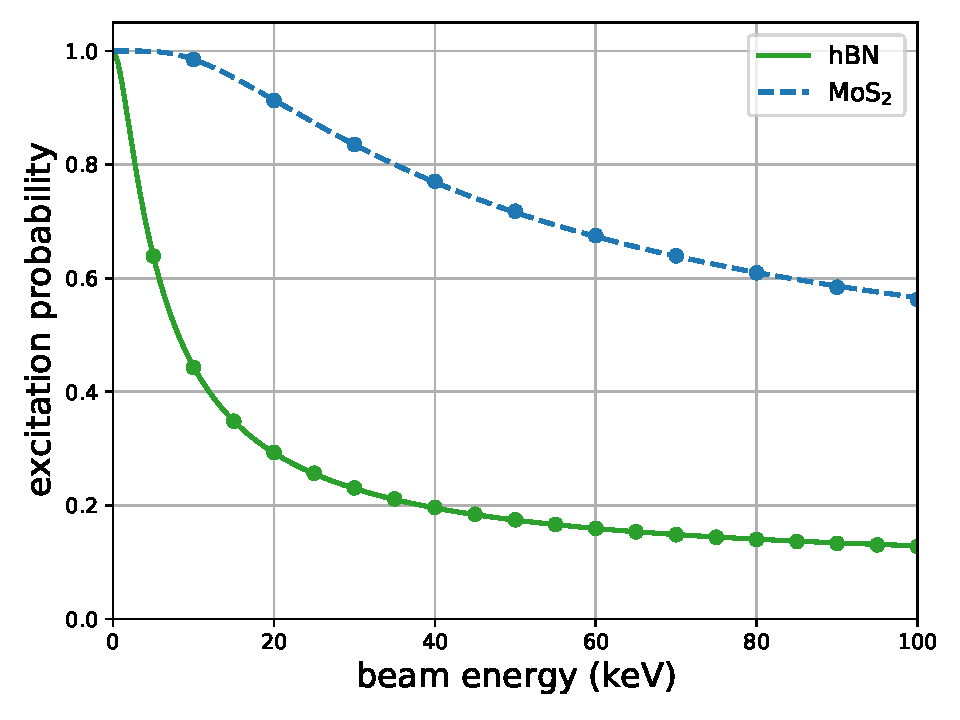
\includegraphics[width=.7\textwidth]{images/pVsEb.pdf}
    \caption{
    The excitation probability decreases with increasing beam energy. MoS$_2$ has a larger excitation probability than hBN does because it has a smaller band gap and more valence states.
    }
    \label{fig:pVsEb}
\end{figure}


Things to discuss
\begin{enumerate}
    \item As the target atom is displaced, the occupied CBM state sinks into the gap and localizes on the displaced atom\cite{Kretschmer2020}.
    \item the excitation lifetime of hBN is ~0.75 ns\cite{Li2016b}.  We can therefore expect that the excitation always lives long enough to reduce the displacement threshold of the affected atom.  The excitation lifetime of MoS$_2$ is much shorter, on the order of a few picoseconds\cite{Korn2011,Lagarde2014,Palummo2015}.  Nonradiative pathways are faster than radiative pathways\cite{Shi2013}, so always assume that the excited electron is at the HOMO while the hole is at the LUMO.  A sputtered sulfur atom takes less than a pico second to leave the vicinity of its pristine site\cite{Yoshimura2018}.  Therefore, we can estimate the likelihood that a beam-induced excitation will facilitate a sputtering event using
    
    \begin{equation}
        P(\text{still excited})
        =
        e^{-t/\tau}
    \end{equation}
    %
    where $\tau$ is the excitation lifetime.
    Are non-radiative pathways more important?
    % \item only consider intraband terms in polarization equation (\ref{eq:chi0}) since the intraband overlap is much greater than the interband overlap in the majority of the BZ.
    \item field theory has been laid out, but it has never been applied to materials
    \item time evolution operator should account for potential
    \item excitation probability is inversely proportional to band gap squared
    \item If $P \ll 1$, the excitation probability is inversely proportional to beam energy, as predicted by Bethe\cite{Kretschmer2020}.  multiple excitations are likely at low beam energies.
    \item The excitation probability is inversely proportional to the square of the band gap
    \item hBN armchair edges are more likely to form\cite{Cretu2015}
    \item excitation probabilities should change with the presence of defects
    \item nonadiabatic electronic evolution can change both the relaxation time
      $\tau$ and the displacement threshold $E_b$.
    \item as we do now the precise relaxation pathway, we plot the sputtering
      cross section for several values of $\tau$ along with the experimental
      date (figure \ref{fig:totCrosshBN.pdf})
\end{enumerate}


\begin{figure}
    \centering
    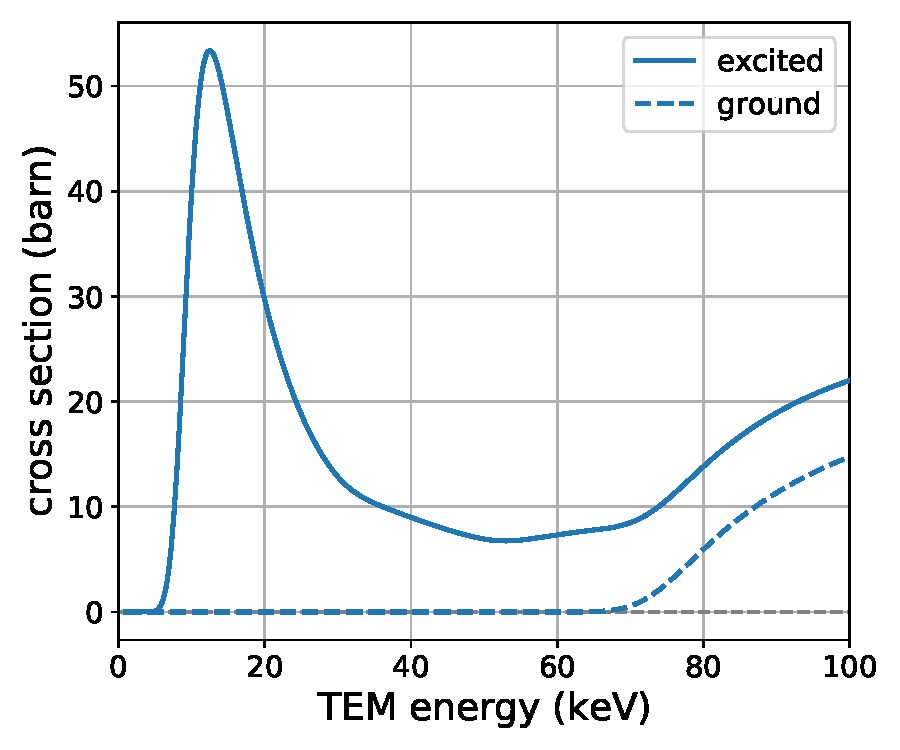
\includegraphics[width=0.7\textwidth]{images/totCrosshBN.pdf}
    \caption{
    Beam-induced excitations in hexagonal boron nitrice (hBN) cause the sputtering rate to peak at beam energies well-below the ground state critical energy.  The dashed line shows the sputtering cross section for ground state hBN, while the solid line accounts for up to three excitations.  A temperature of 300 K was assumed.
    }
    \label{fig:totCrosshBN.pdf}
\end{figure}

%------------------------------- Conclusion ---------------------------------
\section{Conclusion}
%-------------------------------------------------------------------------------

For a given electron beam energy, the sputtering rate is much greater than what is currently predicted by ground state models.
We combine QED scattering theory with DFT orbitals to determine the likelihood of beam induced excitation.  We then show how this excitation probability to calculate the sputtering cross section in hBN in MoS$_2$.

There is room for several improvements to calculating the probability of subsequent excitations.

\begin{enumerate}
    \item Accommodate PAW and ultrasoft pseudopotentials, in the same way done in \cite{Shishkin2006a, Gajdos2006, Paier2005}.
    \item Calculate excited state plane wave coefficients self-consistently using constrained DFT.
    \item consider core excitations and second order electonic excitation effects.  Core excitations are less likely to affect sputtering rates since they have shorter lifetimes and a smaller excitation probability due to the much larger excitation energy.
    \item Include ionization and other electronic responses
    \item spin polarization effects can be accounted for by making $\mathcal{M}$ spin-dependent.  That is, not averaging over spins as is done in equation (\ref{eq:M})
    \item excitations are likely correlated, so that the excitation probability depends on the specific excitations that have already occured.
    \item better treatment of excitation dynamics\cite{Kretschmer2020} and relaxation pathways\cite{}.
    \item In the case of atomic displacement, the beam electron path changes significantly after collision with the nucleus.  This new path would produce a different excitation probability.
    \item different electronic relaxation pathways\cite{Lagarde2014,Kozawa2014,Nie2015,Shi2013a}
\end{enumerate}

% Because the prob (\ref{eq:threeProbs}), the fact that an ex

%------------------------------- Probability ---------------------------------
\section{Methods}
%-------------------------------------------------------------------------------

Density functional theory (DFT)\cite{Hohenberg1964, Kohn1965} was used to determine electronic and ionic structure for all materials from first-principles.  Relaxation calculations were carried using the Vienna ab initio Simulation Package (VASP)\cite{Kresse1996, Kresse1996a} using the projector augmented wave method (PAW)\cite{Blochl1994}.  The plane wave coefficients $C^n_\mathbf{G+k}$ were obtained with Quantum ESPRESSO\cite{Giannozzi2009} utilizing optimized norm-conserving Vanderbilt pseudopotentials\cite{Hamann2013, Schlipf2015}.

Because condition (\ref{eq:interband}) relies on the orthogonality of our Kohn-sham orbitals, the optimized norm-conserving Vanderbilt pseudopotentials\cite{Hamann2013, Schlipf2015} were used to determine all plane wave coefficients.  It is of course possible to extend this method to ultrasoft and projector augmented wave (PAW) \cite{Blochl1994} pseudopotentials using methods laid out in the literature\cite{Shishkin2006a, Gajdos2006, Paier2005}.

%------------------------------- Probability ---------------------------------
\section{Acknowledgements}
DFT and probability calculations were performed in the Center for Compuational
Innovations at Rensselaer Polytechnic Institute and the Livermore Computing
center at Lawrence Livermore National Laboratory.
The authors thank Arkady Krasheninnikov, Tao Yu, and Jon Maienschein for helpful conversations.
%-------------------------------------------------------------------------------

\printbibliography
\end{document}

%------------------------------- Appendix ---------------------------------
% \appendix
% \numberwithin{equation}{section}
% \renewcommand{\theequation}{\thesection.\arabic{equation}}

% \end{document}

% %%%%%%%%%%%%%%%%%%%%%%%%%%%%%%%%%%%%%%%%%%%%%%%%%%%%%%%%%%%%%%%%%%%%%%%%%%%%%%%
% \section{The virtual photon propagator}
% %%%%%%%%%%%%%%%%%%%%%%%%%%%%%%%%%%%%%%%%%%%%%%%%%%%%%%%%%%%%%%%%%%%%%%%%%%%%%%%

% In this section, we formulate how the virtual photon propagator $D_{\mu\nu}$ in equation (\ref{eq:spinors}) depends on the electronic structure of the irradiated material. QED posits that the interaction between charged particles is mediated by the transmission of a virtual photon.  It follows that any electron-electron scattering amplitude includes a multiple of the photon propagator $D_{\mu\nu}(q)$, where $q$ is the momentum of the photon, as is the case in equation (\ref{eq:spinors}).  We have not yet explicitly written the form of the photon propagator.

% Suppose that the transmitted photon behaves like a free particle, i.e., it does not undergo any interactions as it propagates between the two electrons.  For this case, the free photon propagator takes the form\cite{Lancaster2014, Peskin1995}

% \begin{equation}
% \label{eq:D0}
%     D_0^{\mu\nu}(q) = \frac{-ig^{\mu\nu}}{q^2 + i\eta},
% \end{equation}
% %
% where $\eta$ is an infinitesimal positive real number that moves the pole off the real axis.

% The momentum of the virtual photon is that which is transferred to the material electron.  This must satisfy conservation of 4-momentum.

% This form implies that the interaction between the beam and material electrons is ``long-ranged," evident in the fact that the square of the photon momentum $q$ appears alone in the denominator.  As a result, inserting this propagator into the $t$ and $u$ terms in equation (\ref{eq:spinors}) causes the scattering amplitude to blow up as $q$ goes to zero.  Assuming this photon is transmitted in a 2D crystalline system, the smallest allowable $q$ is inversely proportional to the area $A$ of the crystal. This means that $D_0(q)$ increases indefinitely as $A$ increases, so that the assumption of a free virtual photon prohibits the convergence of the scattering amplitude with respect to increasing crystal area. Such a divergence is not an issue for the calculation of the ionic \textit{displacement} cross sections used in the literature \cite{Meyer2012,Susi2016,Yoshimura2018}, as the corresponding displacement \textit{thresholds} prevent small-momentum transfer processes from contributing to ionic displacement.  On the other hand, electronic excitation has no analogous energy barrier, as any change in the momentum representation of a valence band state can break the orthogonality between it and a conduction band state.
% the photon propagator
% Therefore, many computational models drastically underestimate beam-induced atomic displacement rates in insulators.
% calculating the probability of a subsequent excitation requires summing over the excitation probabilities for each initial excitation weighted its probability. While this is nothing more than summation, an exact calculation is currently intractable and beyond the scope of this work.
